
%(BEGIN_QUESTION)
% Copyright 2010, Tony R. Kuphaldt, released under the Creative Commons Attribution License (v 1.0)
% This means you may do almost anything with this work of mine, so long as you give me proper credit

\textit{Destillasjon} er en prosess med kontinuerlig koking og kondensering for å separere blandinger av ulike væsker.  Et praktisk eksempel er separasjon av råolje til flere gasser og væsker (propan, butan, nafta, heksan osv.).  Komponenter med høyere kokepunkt (typisk tettere væsker) samles i bunnen av kolonnen, mens komponenter med lavere kokepunkt (typisk lettere væsker) og gasser samles i toppen.

I denne destillasjonskolonnen måles væskenivået i bunnen med en fortrengertype nivåtransmitter:

$$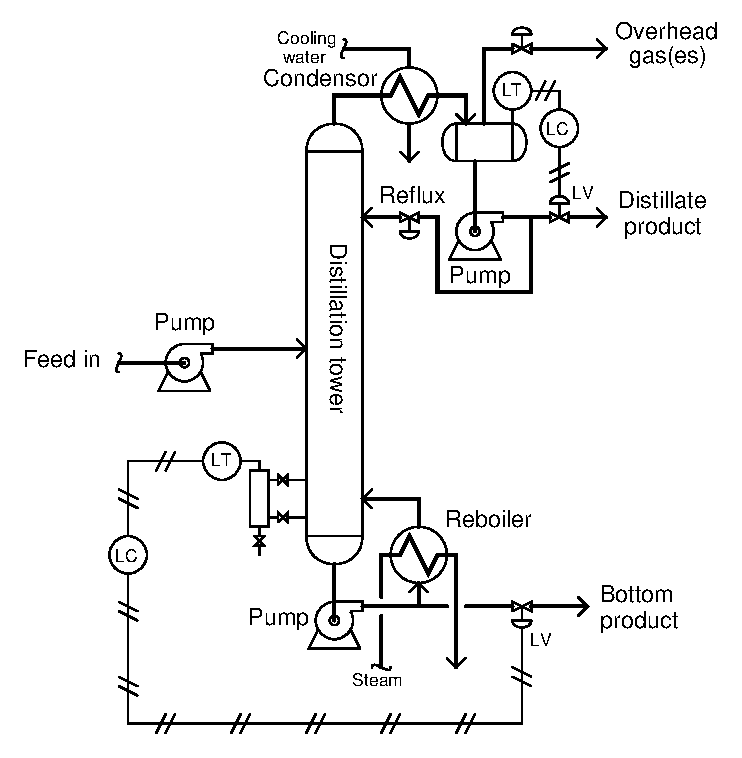
\includegraphics[width=15.5cm]{i00269x01.eps}$$

En instrumenttekniker beregner oppdriftskraften for fortrengeren i dette nivåinstrumentet til 0 pund ved 0\% nivå, og 3.75 pund ved 100\% nivå.  Forklar hvordan du ville kontrollert kalibreringen mens kolonnen var i drift, med disse tallene.

\vskip 20pt \vbox{\hrule \hbox{\strut \vrule{} {\bf Forslag til sokratisk diskusjon} \vrule} \hrule}

\begin{itemize}
\item{} Hvilke sikkerhetsforhold i prosessen må du være oppmerksom på?
\item{} Hvilken \textit{standard} bruker du i kalibreringen (hva kontrollerer du instrumentet mot)?
\item{} Finnes prosessfaktorer som kan skjevstille kalibreringsnøyaktigheten mens instrumentet er i drift?
\end{itemize}

\underbar{file i00269}
%(END_QUESTION)





%(BEGIN_ANSWER)

Ikke glem å kontakte operatør(ene) for prosessen, og få nivåregulatoren satt i manuell modus (eller gjør det selv)!  Bunnproduktnivået i destillasjonskolonnen må styres manuelt under hele kalibreringstesten.

%(END_ANSWER)





%(BEGIN_NOTES)

To hovedmetoder finnes her: \textit{wet} kalibrering eller \textit{dry} kalibrering.  Uansett metode må operatøren først sette nivåregulatoren i manuell modus slik at kalibreringsarbeidet ikke får nivåventilen til å bevege seg ukontrollert.

\vskip 10pt

Ved wet-kalibrering: tøm kammeret og kontroller LRV (zero).  Fyll deretter kammeret helt med bunnprodukt og kontroller URV.

\vskip 10pt

Ved dry-kalibrering: tøm kammeret og kontroller LRV (zero).  Påfør deretter 3.75 pund oppoverkraft på fortrengeren og kontroller URV.


\vfil \eject

En lærerik hendelse innen yrkesetikk og sikkerhet for fortrengerbaserte nivåinstrumenter skjedde på et oljeraffineri der jeg jobbet i 1989.  En Fisher Level-Trol pneumatisk transmitter målte og regulerte butannivå i bunnen av ``debutanizer''-kolonnen i råoljeenheten.  Under oppstart så operatørene et problem: indikasjonen i DCS i kontrollrommet (fra en P/I-omformer på Level-Trol-utgangen) viste mettet høyt nivå, mens feltoperatør verifiserte 0\% nivå i kolonnen via skueglass (LG):

$$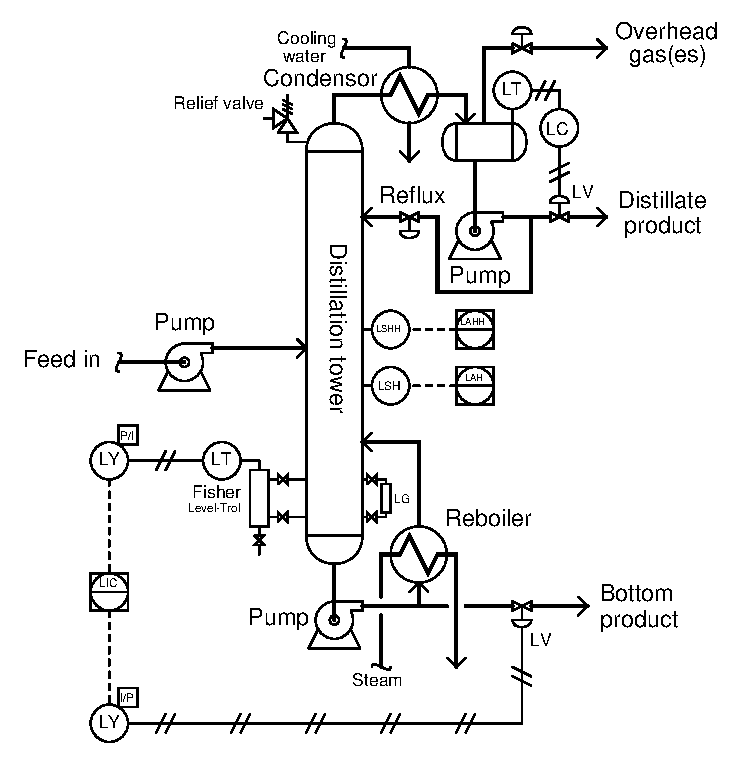
\includegraphics[width=15.5cm]{i00269x02.eps}$$

\vskip 10pt

\filbreak

Hendelsesforløp:

\begin{itemize}
\item{} Operatørene ser LIC vise 105\% nivå i kolonnebunnen.
\item{} En feltoperatør leser 0\% nivå i LG på samme kolonne.
\item{} En instrumenttekniker tilkalles for å reparere Level-Trol-transmitteren.  {\it Hva tror du kan være galt, siden den viser falskt høyt?}
\item{} Det er en kald vinternatt, og teknikeren velger å justere nullpunktet på Level-Trol slik at signalet blir 0\%, likt skueglasset.  {\it Hva er feil med denne handlingen?}
\item{} Teknikeren går tilbake til varm verkstedhall uten å verifisere videre at transmitteren fortsatt måler nivå korrekt.
\item{} Uten at teknikeren vet det er Level-Trol faktisk defekt: fortrengeren har falt av enden av vrirøret, slik at vrirøret står uten belastning.  Da fjærer vrirøret til ``full''-stilling, som ga 105\% fra start.  Justering av nullskruen løste ingenting.
\item{} LIC reagerer på transmitterens 0\%-signal ved å stenge bunnproduktventilen, og butan akkumuleres i kolonnen.
\item{} Når butan akkumuleres, viser den defekte Level-Trol fortsatt 0\%, og LIC holder ventilen stengt.
\item{} Butannivået stiger til LAH-alarm.  Operatørene kvitterer alarmen.
\item{} Butannivået stiger til LAHH-alarm.  Operatørene kvitterer denne også.
\item{} Kolonnen fylles til slutt helt med flytende butan, og innholdet blir inkompressibelt slik at sikkerhetsventilen åpner.
\item{} Flytende butan strømmer ut av sikkerhetsventilen og samler seg på bakken rundt kolonnen i omtrent ett minutt.
\item{} Noe antenner butanen, og den tar fyr.  Debutanizer-kolonnen og åpen sikkerhetsventil står i brann.  Flammen fra sikkerhetsventilen er minst like høy som selve kolonnen.
\item{} Brannmannskap slukker brannen før andre trykkbeholdere overtrykkes.
\item{} Operatørene stenger råoljeenheten.  Enheten står i reparasjon i over en måned (driftstap omtrent \$1 million per dag).
\end{itemize}


\vskip 20pt \vbox{\hrule \hbox{\strut \vrule{} {\bf Forslag til sokratisk diskusjon} \vrule} \hrule}

\begin{itemize}
\item{} Hva gjorde teknikeren feil?
\item{} Hvis du var teknikeren, hva ville du gjort annerledes?
\item{} Hva gjorde operatørene feil?
\item{} Hvis du var en av operatørene, hva ville du gjort annerledes?
\end{itemize}

%INDEX% Measurement, level: displacer (buoyancy)
%INDEX% Process: distillation (generic)

%(END_NOTES)
